
\documentclass[12pt, addpoints]{exam}
\usepackage[utf8]{inputenc}
\usepackage[portuguese]{babel}
\usepackage{multicol}
\usepackage{graphicx}
\usepackage{amsmath}
\usepackage{xcolor}
\usepackage[a4paper, portrait, margin=2cm]{geometry}

\setlength{\columnsep}{1cm}

        \begin{document}

\begin{minipage}[l]{0.5\linewidth}
    \begin{flushleft}
        {\bf \Large Prova bimestral}
    \end{flushleft}
\end{minipage}
\begin{minipage}[r]{0.45\linewidth}
    \begin{flushright}
        {\bf \Large Código: XXXXX}
    \end{flushright}
\end{minipage}
\vspace{0.5cm} \hrule \vspace{0.5cm}
\begin{minipage}{0.75\linewidth}
    Aluno:
\end{minipage}
\begin{minipage}{0.20\linewidth}
    Data: 
\end{minipage}
\vspace{0.5cm} \hrule \vspace{0.5cm}

\begin{questions}
\begin{multicols}{2}
\question[33] 
            Durante sua trajetória uma partícula realizou um trabalho de   -3.28 J. Qual foi a variação da sua energia cinética?
        
\begin{oneparchoices}
\choice -3.15 J\choice -6.42 J\choice 6.5 J\choice -3.28 J\choice -5.08 J\choice 4.99 J\choice -7.6 J\choice -1.72 J\choice -0.08 J\choice 2.9 J\end{oneparchoices}
\question[23] 
            Considere uma partícula de massa    5.05 kg e velocidade    2.23 m/s. Determine a sua energia cinética.
        
\begin{center}
\begin{minipage}[c]{0.75\linewidth}
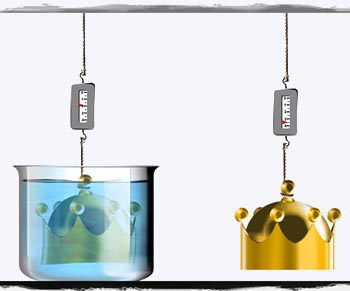
\includegraphics[width=\textwidth]{MWE001.jpg}
\end{minipage}
\end{center}
\begin{oneparchoices}
\choice 61.03 J\choice 104.68 J\choice 284.54 J\choice 325.69 J\choice 40.67 J\choice 33.77 J\choice 7.85 J\choice 12.59 J\choice 36.84 J\choice 54.33 J\end{oneparchoices}
\end{multicols}
\end{questions}
\newpage
\begin{minipage}[l]{0.5\linewidth}
    \begin{flushleft}
        {\bf \Large Prova bimestral}
    \end{flushleft}
\end{minipage}
\begin{minipage}[r]{0.45\linewidth}
    \begin{flushright}
        {\bf \Large Código: XXXXX}
    \end{flushright}
\end{minipage}
\vspace{0.5cm} \hrule \vspace{0.5cm}
\begin{minipage}{0.75\linewidth}
    Aluno:
\end{minipage}
\begin{minipage}{0.20\linewidth}
    Data: 
\end{minipage}
\vspace{0.5cm} \hrule \vspace{0.5cm}

\begin{questions}
\begin{multicols}{2}
\question[33] 
            Durante sua trajetória uma partícula realizou um trabalho de    6.10 J. Qual foi a variação da sua energia cinética?
        
\begin{oneparchoices}
\choice 6.1 J\choice 0.21 J\choice 6.07 J\choice -1.73 J\choice 1.27 J\choice -6.31 J\choice 7.28 J\choice -2.7 J\choice -7.88 J\choice 8.63 J\end{oneparchoices}
\question[23] 
            Considere uma partícula de massa    8.79 kg e velocidade    7.09 m/s. Determine a sua energia cinética.
        
\begin{center}
\begin{minipage}[c]{0.75\linewidth}
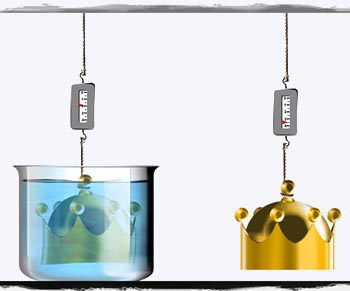
\includegraphics[width=\textwidth]{MWE001.jpg}
\end{minipage}
\end{center}
\begin{oneparchoices}
\choice 801.15 J\choice 445.18 J\choice 39.29 J\choice 100.3 J\choice 137.27 J\choice 330.75 J\choice 220.81 J\choice 31.7 J\choice 101.66 J\choice 26.88 J\end{oneparchoices}
\end{multicols}
\end{questions}
\newpage\end{document}